\subsection{角}\label{subsec:czjh1-1-5}

钟表上的时针与分针,两脚规张开的两脚,它们都给我们以角的形象(图\ref{fig:czjh1-1-21})。

\begin{figure}[htbp]
    \centering
    \begin{minipage}[b]{7cm}
        \centering
        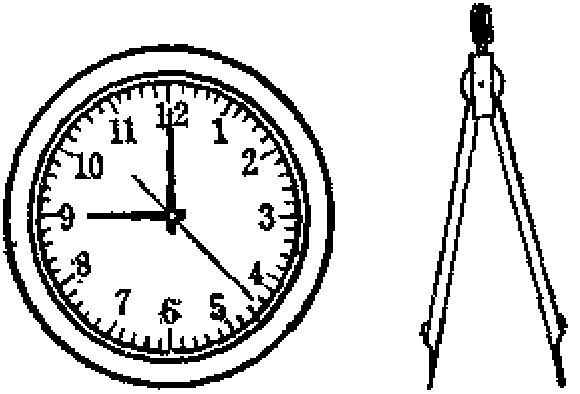
\includegraphics[width=5cm]{../pic/czjh1-ch1-21.png}
        \caption{}\label{fig:czjh1-1-21}
    \end{minipage}
    \qquad
    \begin{minipage}[b]{7cm}
        \centering
        \begin{tikzpicture}
	\begin{scope}
		\tkzDefPoint(0,0){O}
		\tkzDefPoint(0:1.5){A}
		\tkzDefPoint(120:1.5){B}
		\tkzDrawSegments[thick](O,A  O,B)
	\end{scope}

	\begin{scope}[xshift=2.5cm]
		\tkzDefPoint(0,0){O}
		\tkzDefPoint(0:1.5){A}
		\tkzDefPoint(45:1.5){B}
		\tkzDrawSegments[thick](O,A  O,B)
	\end{scope}
\end{tikzpicture}


        \caption{}\label{fig:czjh1-1-22}
    \end{minipage}
\end{figure}

在小学里我们已经学过角,现在我们来看图 \ref{fig:czjh1-1-22} 中的两个图形。
它们都是由两条射线组成的,而且两条射线有公共端点。
这种有公共端点的两条射线所组成的图形叫做\zhongdian{角},
这个公共端点叫做\zhongdian{角的顶点},
这两条射线叫做\zhongdian{角的边}。

我们再来看图 \ref{fig:czjh1-1-23} 甲, 一条射线 $OA$ 由原来的位置,绕着它的端点 $O$ 旋转到另一个位置。
这时,在起始位置的射线 $OA$ 与终止位置的射线 $OB$ 就形成了一个角。
因此,我们也可以把角看成是由一条射线绕着它的端点旋转而成的。
起始位置的射线 $OA$ 叫做\zhongdian{角的始边},
终止位置的射线 $OB$ 叫做\zhongdian{角的终边}。
角的始边旋转到角的终边所经过的平面部分(图 \ref{fig:czjh1-1-23} 乙中的阴影部分)是角的内部,
平面的其余部分是角的外部(图 \ref{fig:czjh1-1-23} 乙中的无阴影部分)。

\begin{figure}[htbp]
    \centering
    \begin{minipage}[b]{6cm}
        \centering
        \begin{minipage}[b]{2.7cm}
            \centering
            \begin{tikzpicture}
	\tkzDefPoint(0,0){O}
	\tkzDefPoint(0:2){A}
	\tkzDefPoint(45:2){B}
	\tkzDrawSegments[thick](O,A  O,B)
	\tkzMarkAngle[-stealth,size=0.5](A,O,B)
	\tkzLabelPoints[below](O, A)
	\tkzLabelPoints[above](B)
\end{tikzpicture}


            \caption*{甲}
        \end{minipage}
        \quad
        \begin{minipage}[b]{2.7cm}
            \centering
            \begin{tikzpicture}
	\tkzDefPoint(0,0){O}
	\tkzDefPoint(0:2){A}
	\tkzDefPoint(45:2){B}
	\tkzDrawSegments[thick](O,A  O,B)
	\tkzFillPolygon[pattern={mylines[angle=65, distance={4pt}]}](A,O,B)
	\tkzMarkAngle[-stealth,size=0.5](A,O,B)
	\tkzLabelPoints[below](O, A)
	\tkzLabelPoints[above](B)
\end{tikzpicture}


            \caption*{乙}
        \end{minipage}
        \caption{}\label{fig:czjh1-1-23}
    \end{minipage}
    \qquad
    \begin{minipage}[b]{8cm}
        \centering
        \begin{minipage}[b]{4cm}
            \centering
            \begin{tikzpicture}
	\tkzDefPoints{0/0/O, 1.5/0/A, -1.5/0/B}
	\tkzDrawLine[add=0.1 and 0.1](B,A)
	\tkzMarkAngle[-stealth,size=0.5](A,O,B)
	\tkzDrawPoint[fill=black](O)
	\tkzLabelPoints[below](O, A, B)
\end{tikzpicture}


            \caption*{甲}
        \end{minipage}
        \quad
        \begin{minipage}[b]{3cm}
            \centering
            \begin{tikzpicture}
	\tkzDefPoints{0/0/O, 1.5/0/A, 1.5/0/B, -1.5/0/B'}
	\tkzDrawLine[add=0 and 0.3](O,A)
	\tkzMarkAngle[size=0.5](A,O,B')
	\tkzMarkAngle[-stealth,size=0.5](B',O,B)  % euclide 不支持360的角,所以分两段来绘制
	\tkzDrawPoint[fill=black](O)
	\tkzLabelPoints[below](O)
	\tkzLabelPoint[below](B){$(B)$}
	\tkzLabelPoints[above](A)
\end{tikzpicture}


            \caption*{乙}
        \end{minipage}
        \caption{}\label{fig:czjh1-1-24}
    \end{minipage}
\end{figure}

一条射线由原来的位置 $OA$, 绕着它的端点 $O$ 旋转至位置 $OB$,
当 $OB$ 和 $OA$ 成一条直线时,所成的角叫做\zhongdian{平角}( 图 \ref{fig:czjh1-1-24} 甲);
再旋转下去,当终边 $OB$ 与始边 $OA$ 重合时,所成的角叫做\zhongdian{周角}( 图 \ref{fig:czjh1-1-24} 乙)。

本书今后所说的角,除非特别注明,都是指小于平角的角。

我们用符号 “$\angle$” 来表示角。
一个角可以用三个大写字母来表示,就是在角的两条边上各取一个点,把表示顶点的字母写在这两个点的字母中间。
如图 \ref{fig:czjh1-1-23} 中的角可以记作 $\angle AOB$(读作 “角$AOB$”) 或 $\angle BOA$;
又如,图 \ref{fig:czjh1-1-25} 甲中的三个角可以分别记作 $\angle AOB$、$\angle BOC$、$\angle AOC$
或 $\angle BOA$、$\angle COB$、$\angle COA$。

\begin{figure}[htbp]
    \centering
    \begin{minipage}[b]{4cm}
        \centering
        \begin{tikzpicture}
	\tkzDefPoints{0/0/O, 2/0/A, 1.5/1.3/B, 1.2/1.8/C}
	\tkzDrawSegments(O,A  O,B  O,C)
	\tkzLabelPoints[left](O)
	\tkzLabelPoints[right](A, B, C)
\end{tikzpicture}


        \caption*{甲}
    \end{minipage}
    \qquad
    \begin{minipage}[b]{4cm}
        \centering
        \begin{tikzpicture}
	\tkzDefPoints{0/0/B, 1.3/1.3/A, 2/0/C}
	\tkzDrawLines[add=0.2 and 0.2](A,B  B,C  C,A)
	\tkzLabelPoints[above](A)
	\tkzLabelPoints[below](B, C)
	\tkzMarkAngles[size=0.3](B,A,C  C,B,A  A,C,B)
	\tkzLabelAngle[pos=0.5](B,A,C){$\alpha$}
	\tkzLabelAngle[pos=0.5](C,B,A){$\beta$}
	\tkzLabelAngle[pos=0.5](A,C,B){$\gamma$}
\end{tikzpicture}


        \caption*{乙}
    \end{minipage}
    \begin{minipage}[b]{4cm}
        \centering
        \begin{tikzpicture}
	\tkzDefPoints{0/0/A, 2/1.4/B, 2/0/C, 0/1.4/D}
	\tkzInterLL(A,B)(C,D)  \tkzGetPoint{O}
	\tkzDrawSegments(A,B  C,D)
	\tkzMarkAngles[size=0.3](D,O,A  C,O,B)
	\tkzLabelAngle[pos=0.5](D,O,A){$1$}
	\tkzLabelAngle[pos=0.5](C,O,B){$2$}
	\tkzLabelPoints[below](A, C, O)
	\tkzLabelPoints[above](B, D)
\end{tikzpicture}


        \caption*{丙}
    \end{minipage}
    \caption{}\label{fig:czjh1-1-25}
\end{figure}

以某一点为顶点的角只有一个时,这个角也可以用表示这个点的字母来表示。
如图 \ref{fig:czjh1-1-23} 中的 $\angle AOB$ 也可以记作 $\angle O$,
但图 \ref{fig:czjh1-1-25} 甲中的三个角不能记作 $\angle O$。


角还可以用一个小写希腊字母或一个数字写在角的内部靠近顶点处,并加上弧线来表示。
如图 \ref{fig:czjh1-1-25} 乙中的三个角可以分别记作 $\angle \alpha$、$\angle \beta$、 $\angle \gamma$,
  图 \ref{fig:czjh1-1-25} 丙中的 $\angle DOA$、 $\angle COB$ 可以分别记作 $\angle 1$、 $\angle 2$。



\begin{lianxi}

\xiaoti{(口答) 指出图中的角的顶点和边;并用几不同的记法来表示图中的角。}

\begin{figure}[htbp]
    \centering
    \begin{minipage}[b]{4cm}
        \centering
        \begin{tikzpicture}
	\tkzDefPoints{0/0/A, 2/0/B, 1.8/1/C}
	\tkzDrawSegments(A,B  A,C)
	\tkzMarkAngle[size=0.5](B,A,C)
	\tkzLabelAngle[pos=0.8](B,A,C){$\alpha$}
	\tkzLabelPoints[below](A, B)
	\tkzLabelPoints[above](C)
\end{tikzpicture}


        \caption*{(第 1 题)}
    \end{minipage}
    \qquad
    \begin{minipage}[b]{4cm}
        \centering
        \begin{tikzpicture}
	\tkzDefPoints{0/0/O, 2/-0.2/B, 1.3/1.2/A, 2.3/0.3/D}
	\tkzInterLL(A,B)(O,D)  \tkzGetPoint{C}
	\tkzDrawLines[add=0 and 0.2](O,A  O,B)
	\tkzDrawSegment(O,D)
	\tkzDrawLines[add=0.2 and 0.2](A,B)
	\tkzLabelPoints[left](O)
	\tkzLabelPoints[right](A,D)
	\tkzLabelPoints[below left](B)
	\tkzLabelPoints[above, xshift=0.3em](C)
\end{tikzpicture}


        \caption*{(第 3 题)}
    \end{minipage}
    \begin{minipage}[b]{4cm}
        \centering
        \begin{tikzpicture}
	\tkzDefPoints{0/0/D, 1/0/E, 2/0/F}
	\tkzDrawLines[add=0.3 and 0.3](D,F)
	\tkzDrawPoints[fill=black](D, E, F)
	\tkzLabelPoints[above](D, E, F)
\end{tikzpicture}


        \caption*{(第 4 题)}
    \end{minipage}
\end{figure}

\xiaoti{(口答) 用三个大写字母分别表示图 \ref{fig:czjh1-1-25} 乙中的三个角。}

\xiaoti{(口答) 图中以点 $O$ 为顶点的角有几个? 怎样表示这些角? 以点 $C$ 为顶点的角呢?}

\xiaoti{}%
\begin{xiaoxiaotis}%
    \xxt[\xxtsep]{指出图中以 $E$ 为顶点的平角的两条边,并用三个大写字母表示这个平角。}

    \xxt{一条直线可以看成一个平角吗?为什么?}

\end{xiaoxiaotis}

\end{lianxi}

